\documentclass[12pt]{article}

\usepackage[english]{babel}
\usepackage[utf8x]{inputenc}
\usepackage{amsmath}
\usepackage{enumitem}
\usepackage{graphicx}
\usepackage{ulem}
\usepackage{caption}
\usepackage{placeins}
\usepackage[usenames,dvipsnames]{color}
\usepackage[colorinlistoftodos]{todonotes}
\usepackage{listings}
\usepackage{fixltx2e}
\usepackage{scrpage2}
\usepackage{lastpage}
\clearscrheadfoot
\pagestyle{scrheadings}
\usepackage{glossaries}
\usepackage[
top    = 2.75cm,
bottom = 2.00cm,
left   = 2.50cm,
right  = 2.00cm]{geometry}
\setcounter{secnumdepth}{4}


\makeglossaries

\newglossaryentry{glossaryVerweis} {name=abkuerzung, description={Langer Name}}

\newcommand{\executeiffilenewer}[3]{%
\ifnum\pdfstrcmp{\pdffilemoddate{#1}}%
{\pdffilemoddate{#2}}>0%
{\immediate\write18{#3}}\fi%
}
\newcommand{\includesvg}[2]{%
\executeiffilenewer{#1.svg}{#1.pdf}%
{rsvg-convert -f pdf #1.svg > #1.pdf}%
\includegraphics[width=1\textwidth]{#1.pdf}}%



\begin{document}
\begin{titlepage}
\begin{center}
% Oberer Teil der Titelseite:

\includegraphics[width=0.5\textwidth]{images/logo}\\[1cm]    

\textsc{\LARGE Technologisches Gewerbe Museum}\\[1.5cm]

% Title
\rule{12cm}{1mm}
{ \huge \bfseries  \\\large FACH\\ \huge Aufgaben-Titel \\[0.4cm] }

\rule{12cm}{1mm}

% Author and supervisor
\noindent 
\vspace{5cm}

\begin{center}
\large
Author: 
Nachname1 \textsc{Vorname1} \&
Nachname2 \textsc{Vorname2}
\end{center}

\vfill

% Bottom of the page
{\large \today}

\end{center}
\end{titlepage}

\tableofcontents


%HEADER AND FOOTER
\pagenumbering{arabic}
\ohead{\headmark}
\automark{section}
\ifoot{© Authors}
\ofoot{\pagemark ~of \pageref{LastPage}}

\newpage
\section{Introduction for everybody}
So I guess the purpose of this document is quite clear. Everybody can share his or her knowledge in Latex into this document. \\
It can then be used for any Borko-Tasks and stuff. \\
The language of documentation is English, so that everybody and their grandma can use this document.
Also the basic things should be described somewhere, so that also beginners can make a use of this document. \\ \\
Furthermore, the .tex file counts as a documentation and not the output into pdf. If someone wants to change this, they are welcome to do so tho! This means, that normally, the user of this document will have to read the .tex file rather than the pdf. \\ \\
Collaborators can add their names here: \\
\textbf{Hannah Siegel}(hsiegel-tgm) \\
\newpage
\section{Basic Latex Commands}
\subsection{Text Formatting}
\textit{italic} \\
\emph{emph} \\
\textbf{bold} \\
\texttt{code} \\
\underline{underlinded} \\
\dashuline{dashed underlined} \\
\subsection{Alignment of text}

\subsection{Colors}
\color{red} 
red \\
\textcolor{blue}{text} \\
red \\
\color{OrangeRed} OrangeRed \\
\color{black} red \\
\subsubsection{Defining customized colors}
\definecolor{rgb}{RGB}{255,100,200} 
\definecolor{dark-gray}{gray}{0.1} 
\color{rgb} test \\
\color{dark-gray} test
\color{black} 
\newpage
\section{Graphics}
\subsection{Including graphics using figures}
\begin{figure}[here!]
\centering
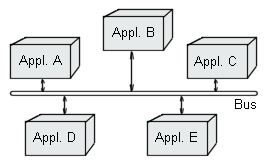
\includegraphics[width=0.6\textwidth]{images/eai2.png}
\caption{caption1}
\end{figure}
\listoffigures
\newpage

\subsection{Including svg using rsvg-convert}
If you want to insert svg you will need to add this to the PdfLaTex-Command:\\
\texttt{\color{red} --shell-escape --enable-write18 \%.tex }
\begin{figure}[here!]
\centering
\includesvg{images/uml}
\caption{svg}
\end{figure}
\FloatBarrier

\listoffigures
\newpage

\section{References and referencing}
\subsection{Easy Bibliography}
\begin{thebibliography}{56}

\bibitem{name}
   \textbf{Who}, When\\
  \textit{url}
  \newline last used: dd.mm.yyyy, hh:mm
 
 \bibitem{example} 
  \textbf{Mister Super-genious}, Answer from 20.01.2015\\
  \textit{http://www.stackoverflow.com/question}
  \newline last used: 22.10.2014, 21:00
\end{thebibliography}

This source can be cited using:
\begin{lstlisting}
 \cite{name}
\end{lstlisting}
 \cite{name}

\subsection{More complicated/'better' Bibliography}
''I'm a cite from a book'' \cite{bk_key}  \\\\
Some content-related cite \cite{up_key} \\\\
\textbf{\color{red}Entries in your bib-file you don't relate with a \textbackslash{}cite aren't listed!}
\newline
\newline
\bibliography{sources} 
\bibliographystyle{alpha}
\newpage

\subsection{Referencing}
Referencing in Latex is quite easy, all that has to be done is:
\begin{enumerate}
\item Define the 'point-of-reference' with: 
\begin{lstlisting}
\label{type:name}
\end{lstlisting}
\item Refer to the item using: 
\begin{lstlisting}
\ref{type:name}
\end{lstlisting}
\end{enumerate}
\newpage
\section{Document and Layout}
\subsection{Minipages}
Whenever you want to layout your document a little bit more, the use of minipages would be great!
Take care: text width within a minipage always depends on the size of the minipage.
\begin{figure}[here!]
\centering
\begin{minipage}[h]{0.3\textwidth}
\centering
    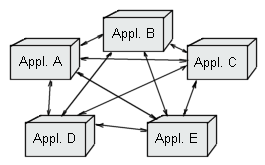
\includegraphics[width=1.0\textwidth]{images/eai0.png}
    \caption{Star-topology}
    \label{fig:eai0}
\end{minipage}
\begin{minipage}[h]{0.3\textwidth}
\centering
    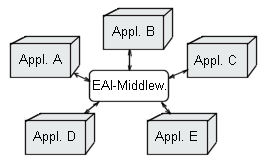
\includegraphics[width=1.0\textwidth]{images/eai1.png}
    \caption{Hub-topology}
    \label{fig:eai1}
\end{minipage}
\begin{minipage}[h]{0.3\textwidth}
\centering
    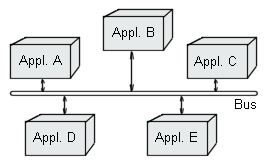
\includegraphics[width=1.0\textwidth]{images/eai2.png}
    \caption{Bus-topology}
    \label{fig:eai2}
\end{minipage}
\end{figure}
\FloatBarrier
\subsection{Letting some space free}
If you wish to leave some space free in your document, use the vspace command
\begin{lstlisting}
\vspace{0.1\textheight}
\end{lstlisting}
This looks like this:
\vspace{0.1\textheight}
\subsection{The Usage of Itemize and co}
\subsubsection{Itemize}
\begin{itemize}
\item item1
\item item2
\end{itemize}
\subsubsection{enumerate}
\begin{enumerate}
\item enumerate1
\item enumerate2
\end{enumerate}
\subsubsection{description}

\begin{description}
\item[First] The first item
\item[Second] The second item
\end{description}

\subsubsection{Nested items}

\begin{enumerate}
  \item The first item
  \begin{enumerate}
    \item Nested item 1
    \item Nested item 2
  \end{enumerate}
  \item The second item
\end{enumerate}

\subsubsection{enumerate using letters}

\begin{enumerate}[label=(\alph*)]
\item an apple
\item a banana
\item a carrot
\item a durian
\end{enumerate}
\vspace{0.05\textheight}
\begin{enumerate}[label=(\Alph*)]
\item an apple
\item a banana
\item a carrot
\item a durian
\end{enumerate}
\vspace{0.05\textheight}
\begin{enumerate}[label=(\roman*)]
\item an apple
\item a banana
\item a carrot
\item a durian
\end{enumerate}

\newpage
\section{Tables}
\subsection{Table generator}
For Tables in latex, there is the possibility to use table generators. Simply google this.
\\ \\
Still, the following things should be thought of:
\\
\begin{itemize}
\item the width of a table can be set using 
\begin{lstlisting}
p{0.4\textwidth}
\end{lstlisting}
\end{itemize}

Please note: a default table for the working time can be found in the other document.


\newpage
\section{How to include Code}

\newpage
\section{Important Things, Bugs, Useful Hits ...}
\subsection{Float Barriers}



\subsection{Glossaries}
First of all the entry needs to be defined on the top of the document:
\begin{lstlisting}
\newglossaryentry{cpu} {name=CPU, description={Central Processing Unit}}
\end{lstlisting}
Aterwards, the glossarie entry can be reffered to using:
\begin{lstlisting}
\gls{cpu}
\end{lstlisting}
The glossaries are printed out when you use: 
\begin{lstlisting}
\printglossaries
\end{lstlisting}
Take care: ! I use texmaker and sometimes I have to run this on my command line:
\begin{lstlisting}
 makeglossaries <dokumentenname> ausfuehren
\end{lstlisting}


\newpage

\listoftables
\listoffigures
\printglossaries

\end{document}
